\documentclass[11pt,a4paper]{article}

% ---------------------------------------------------------------------------
% Packages
% ---------------------------------------------------------------------------
\usepackage[utf8]{inputenc}
\usepackage[T1]{fontenc}
\usepackage[english]{babel}
\usepackage{amsmath,amssymb}
\usepackage[version=4]{mhchem}
\usepackage{graphicx}
\usepackage{booktabs}
\usepackage{siunitx}
\usepackage{caption}
\usepackage[hidelinks]{hyperref}
\usepackage{fancyhdr}
\usepackage{lastpage}
\usepackage{geometry}
\geometry{a4paper,margin=2.5cm}

% ---------------------------------------------------------------------------
% Header / footer to mirror the reference report
% ---------------------------------------------------------------------------
\pagestyle{fancy}
\fancyhf{}
\renewcommand{\headrulewidth}{0.4pt}
\renewcommand{\footrulewidth}{0.4pt}
\fancyfoot[C]{Computer Methods in Combustion \quad Page \thepage\ of \pageref{LastPage}}

\setlength{\parindent}{0pt}
\setlength{\parskip}{0.6em}

\sisetup{per-mode=symbol}

% ---------------------------------------------------------------------------
\begin{document}

% ===========================================================================
% Title page
% ===========================================================================
\thispagestyle{empty}
\begin{center}
\vspace*{1.5cm}

{\large Jan Kalak 333459}\\[0.4cm]

{\large Warsaw University of Technology}\\[0.2cm]
{\large Faculty of Power and Aeronautical Engineering}\\[0.2cm]
{\large Computer Methods in Combustion}\\[2.5cm]

{\Large\bfseries Effect of hydrogen enrichment on the ignition delay,
laminar flame speed and NO\textsubscript{x} emissions of methane--air
mixtures under aero gas turbine combustor conditions}\\[2.5cm]

{\large Warsaw, summer semester 2026}

\vfill
\end{center}
\clearpage

% ===========================================================================
% Abstract
% ===========================================================================
\thispagestyle{fancy}
\section*{Abstract}
This work quantifies how blending hydrogen into methane changes three
combustion quantities of direct relevance to an aero gas turbine combustor:
the auto-ignition delay time, the laminar burning velocity and the
NO\textsubscript{x} emission index. All calculations are performed with the
Cantera library and the GRI-Mech~3.0 reaction mechanism. The hydrogen
content is specified as a fraction of the chemical energy of the fuel, which
is the physically meaningful variable for a fuel-substitution
(decarbonisation) scenario. Parametric studies are carried out over the
initial temperature, pressure, equivalence ratio and hydrogen fraction.
The results show that hydrogen markedly shortens the ignition delay and
strongly raises the flame speed, but that the accompanying rise in flame
temperature produces a steep, near-exponential increase in thermal
NO\textsubscript{x}. The choice of GRI-Mech~3.0 across the whole blend range
is validated against a dedicated detailed H\textsubscript{2}/O\textsubscript{2}
mechanism, with agreement better than \SI{3.3}{\percent} for the flame speed
and better than \SI{0.1}{\percent} for the ignition delay of pure hydrogen.

% ===========================================================================
% Contents (manual, to match the reference layout)
% ===========================================================================
\vspace{1cm}
\section*{Contents}
\begin{tabbing}
\hspace{0.6cm}\=\hspace{9.5cm}\=\kill
1 \> Introduction \> 3 \\[2pt]
2 \> State of the art \> 3 \\[2pt]
3 \> Model description \> 4 \\[2pt]
\> \hspace{0.4cm} 3.1 \quad Fuel blend definition \> 4 \\[2pt]
\> \hspace{0.4cm} 3.2 \quad Ignition delay \> 5 \\[2pt]
\> \hspace{0.4cm} 3.3 \quad Laminar burning velocity \> 5 \\[2pt]
\> \hspace{0.4cm} 3.4 \quad NO\textsubscript{x} emissions and flame temperature \> 5 \\[2pt]
4 \> Results \> 6 \\[2pt]
\> \hspace{0.4cm} 4.1 \quad Ignition delay \> 6 \\[2pt]
\> \hspace{0.4cm} 4.2 \quad Laminar burning velocity \> 7 \\[2pt]
\> \hspace{0.4cm} 4.3 \quad NO\textsubscript{x} emissions \> 8 \\[2pt]
\> \hspace{0.4cm} 4.4 \quad Mechanism validation \> 10 \\[2pt]
5 \> Conclusions \> 11 \\[2pt]
\end{tabbing}
\clearpage

% ===========================================================================
% 1. Introduction
% ===========================================================================
\section{Introduction}

Hydrogen is one of the leading candidates for the decarbonisation of gas
turbine combustion. Because it contains no carbon, replacing part of a
hydrocarbon fuel with hydrogen reduces the carbon dioxide produced per unit
of energy released, and in the limit of pure hydrogen eliminates it entirely.
For aero gas turbines this is particularly attractive, but it raises a
practical question: how does the substitution change the combustion
behaviour the engine was designed around?

Three quantities capture most of what matters for combustor design and
operation. The \emph{ignition delay} governs relight at altitude and the
stability of the reaction zone. The \emph{laminar burning velocity} sets the
characteristic flame scale and is closely tied to flashback and blow-off
limits. The \emph{NO\textsubscript{x} emission} determines whether the engine
meets increasingly strict emission regulations. Hydrogen affects all three,
and not always in the same direction, so a quantitative picture of the
trade-offs is needed.

The aim of this project is to compute these three quantities for
methane--hydrogen blends across the full range from pure methane to pure
hydrogen, under conditions representative of an aero gas turbine combustor,
and to identify the dominant trends and the trade-offs they imply. All
calculations are performed with Cantera, an open-source chemical-kinetics
library, using the GRI-Mech~3.0 reaction mechanism.

% ===========================================================================
% 2. State of the art
% ===========================================================================
\section{State of the art}

Methane is the principal component of natural gas and a well-characterised
gas turbine fuel, and its combustion chemistry is described accurately by
established mechanisms such as GRI-Mech~3.0, which was optimised against a
large body of natural-gas combustion data and includes the nitrogen
sub-chemistry required for NO\textsubscript{x} prediction. Hydrogen has a far
higher reactivity, a much larger laminar burning velocity and a higher
adiabatic flame temperature than methane at the same equivalence ratio, all
of which make hydrogen-enriched flames more prone to thermal
NO\textsubscript{x} formation while also improving ignition and stability.

The dominant NO\textsubscript{x} pathway in lean, high-temperature gas
turbine combustion is the thermal (Zeldovich) route, in which atomic oxygen
and nitrogen react at high temperature to form nitric oxide. Because the rate
of this route depends exponentially on temperature, even a moderate increase
in flame temperature translates into a large increase in NO\textsubscript{x}.
Lean operation, which lowers the flame temperature, is therefore the standard
lever for keeping NO\textsubscript{x} within limits, and it is the central
tension when hydrogen, which raises the flame temperature, is introduced.

This study treats the methane--hydrogen system parametrically and uses a
single, internally consistent mechanism over the whole blend range so that
the trends are not confounded by mechanism changes. The validity of that
choice at the pure-hydrogen end is examined explicitly in
Section~\ref{sec:validation}.

% ===========================================================================
% 3. Model description
% ===========================================================================
\section{Model description}

All three quantities are computed with Cantera and the GRI-Mech~3.0
mechanism (53 species, 325 reactions). The code is organised into three
independent modules, one per quantity, that share a common module defining
the fuel blend and the mixture state. Air is modelled as
\ce{O2}:\ce{N2}~=~1:3.76 by mole.

\subsection{Fuel blend definition}

The hydrogen content of the blend is specified as a fraction $x_E$ of the
\emph{chemical energy} supplied by hydrogen, not as a mole fraction. This is
the meaningful variable for the substitution question ``what happens if a
fraction $x_E$ of the fuel energy is provided by hydrogen?''. If $n_{\ce{H2}}$
and $n_{\ce{CH4}}$ are the molar amounts of the two fuels and $\mathrm{LHV}$
denotes the molar lower heating value, then
%
\begin{equation}
x_E = \frac{n_{\ce{H2}}\,\mathrm{LHV}_{\ce{H2}}}
{n_{\ce{H2}}\,\mathrm{LHV}_{\ce{H2}} + n_{\ce{CH4}}\,\mathrm{LHV}_{\ce{CH4}}},
\end{equation}
%
with $\mathrm{LHV}_{\ce{CH4}}=\SI{802.3}{\mega\joule\per\kilo\mole}$ and
$\mathrm{LHV}_{\ce{H2}}=\SI{241.8}{\mega\joule\per\kilo\mole}$. Inverting this
relation gives the mole fractions used to set the Cantera mixture. Because
hydrogen carries much less energy per mole than methane, a given energy
fraction corresponds to a substantially larger mole fraction: an energy share
of \SI{30}{\percent} hydrogen, for instance, is close to \SI{59}{\percent} of
the moles. Table~\ref{tab:blend} lists the mapping.

\begin{table}[h]
\centering
\caption{Mole fractions of the \ce{CH4}/\ce{H2} blend corresponding to a
given hydrogen energy fraction $x_E$.}
\label{tab:blend}
\begin{tabular}{ccc}
\toprule
$x_E$ [\%] & $X_{\ce{CH4}}$ & $X_{\ce{H2}}$ \\
\midrule
0   & 1.000 & 0.000 \\
10  & 0.731 & 0.269 \\
30  & 0.413 & 0.587 \\
50  & 0.232 & 0.768 \\
70  & 0.114 & 0.886 \\
90  & 0.032 & 0.968 \\
100 & 0.000 & 1.000 \\
\bottomrule
\end{tabular}
\end{table}

\subsection{Ignition delay}

The auto-ignition delay is computed in an adiabatic, constant-volume reactor
(Cantera \texttt{IdealGasReactor}), which corresponds to the classical
shock-tube definition. The homogeneous mixture is integrated in time and the
ignition delay $\tau_{ign}$ is taken as the instant of maximum
temperature-rise rate, $\mathrm{d}T/\mathrm{d}t|_{\max}$. This definition is
robust and mechanism-independent. The delay is studied as a function of the
initial temperature ($900$--$\SI{1400}{\kelvin}$), the initial pressure
($1$--$\SI{40}{\bar}$) and the hydrogen energy fraction, at a lean
equivalence ratio of $\phi=0.7$.

\subsection{Laminar burning velocity}

The laminar burning velocity is obtained from a one-dimensional,
freely-propagating, adiabatic premixed flame (Cantera \texttt{FreeFlame})
with mixture-averaged transport and adaptive grid refinement. $S_L$ is the
unburned-gas inlet velocity of the converged solution. The flames are solved
at an unburned temperature of \SI{450}{\kelvin} and a pressure of
\SI{5}{\bar}, as a function of equivalence ratio ($0.5$--$1.4$) and hydrogen
energy fraction. Successive points in a sweep are solved by continuation,
reusing the previous converged profile as the initial guess.

\subsection{NO\textsubscript{x} emissions and flame temperature}

The NO\textsubscript{x} calculation proceeds in two steps. First the fresh
charge is brought to its constant-pressure adiabatic equilibrium state, which
fixes the burned-gas temperature $T_{ad}$ and the major-species and radical
pool. The nitrogen species are then reset to zero and the hot products are
integrated kinetically at constant pressure for a residence time of
\SI{5}{\milli\second}, representative of a gas turbine primary zone. This
yields the NO formed within the available residence time, which is more
realistic than the chemical-equilibrium value because thermal NO formation is
rate-limited. The result is reported as an emission index $\mathrm{EINOx}$, in
grams of \ce{NO2}-equivalent per kilogram of fuel, with all NO converted to an
equivalent mass of \ce{NO2}. The study is performed at \SI{700}{\kelvin} and
\SI{20}{\bar} as a function of equivalence ratio ($0.5$--$1.3$) and hydrogen
fraction.

% ===========================================================================
% 4. Results
% ===========================================================================
\section{Results}

In every figure the curves are labelled by the hydrogen energy fraction,
from \SI{0}{\percent} (pure methane) to \SI{100}{\percent} (pure hydrogen).

\subsection{Ignition delay}

Figure~\ref{fig:ign-T} shows the ignition delay as a function of initial
temperature in Arrhenius form. For every blend the data fall on a near-straight
line in $\log\tau_{ign}$ versus $1/T_0$, confirming Arrhenius-type behaviour.
For pure methane the delay falls from about \SI{294}{\milli\second} at
\SI{900}{\kelvin} to a fraction of a millisecond at \SI{1400}{\kelvin};
hydrogen-rich blends ignite far faster and the separation between the curves
widens with temperature.

\begin{figure}[h]
\centering
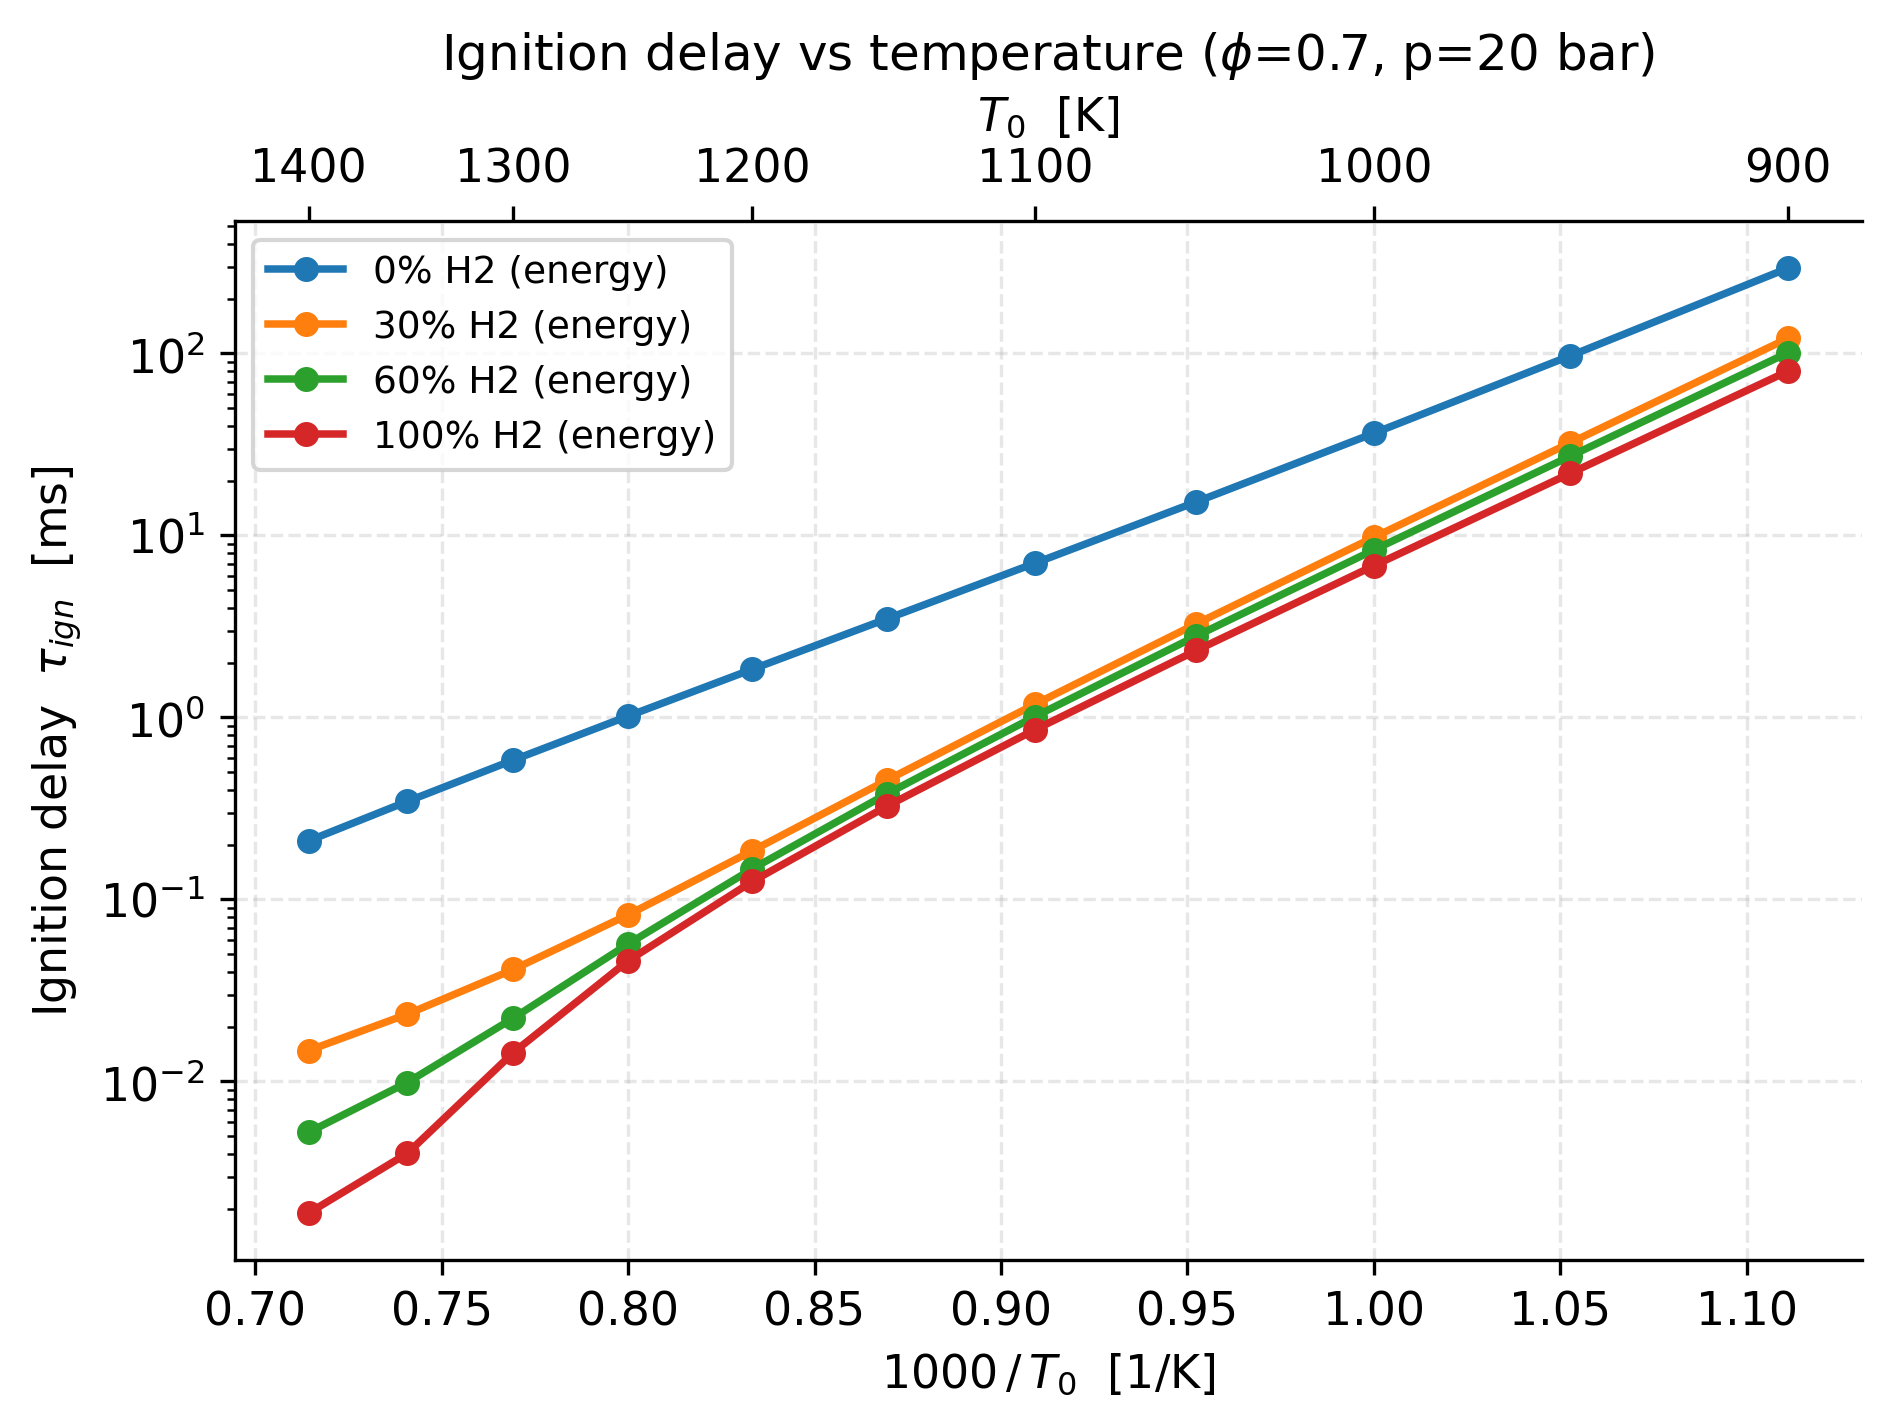
\includegraphics[width=0.78\textwidth]{figures/ignition_T_sweep.png}
\caption{Ignition delay versus initial temperature for different hydrogen
energy fractions ($\phi=0.7$, $p=\SI{20}{\bar}$).}
\label{fig:ign-T}
\end{figure}

The effect of pressure is shown in Figure~\ref{fig:ign-p}. Increasing the
pressure shortens the ignition delay for all blends, as expected from the
higher collision frequency. For methane the dependence is close to a single
power law over the whole range, whereas the hydrogen-rich blends show the
non-monotonic behaviour characteristic of the hydrogen explosion limits at
low pressure.

\begin{figure}[h]
\centering
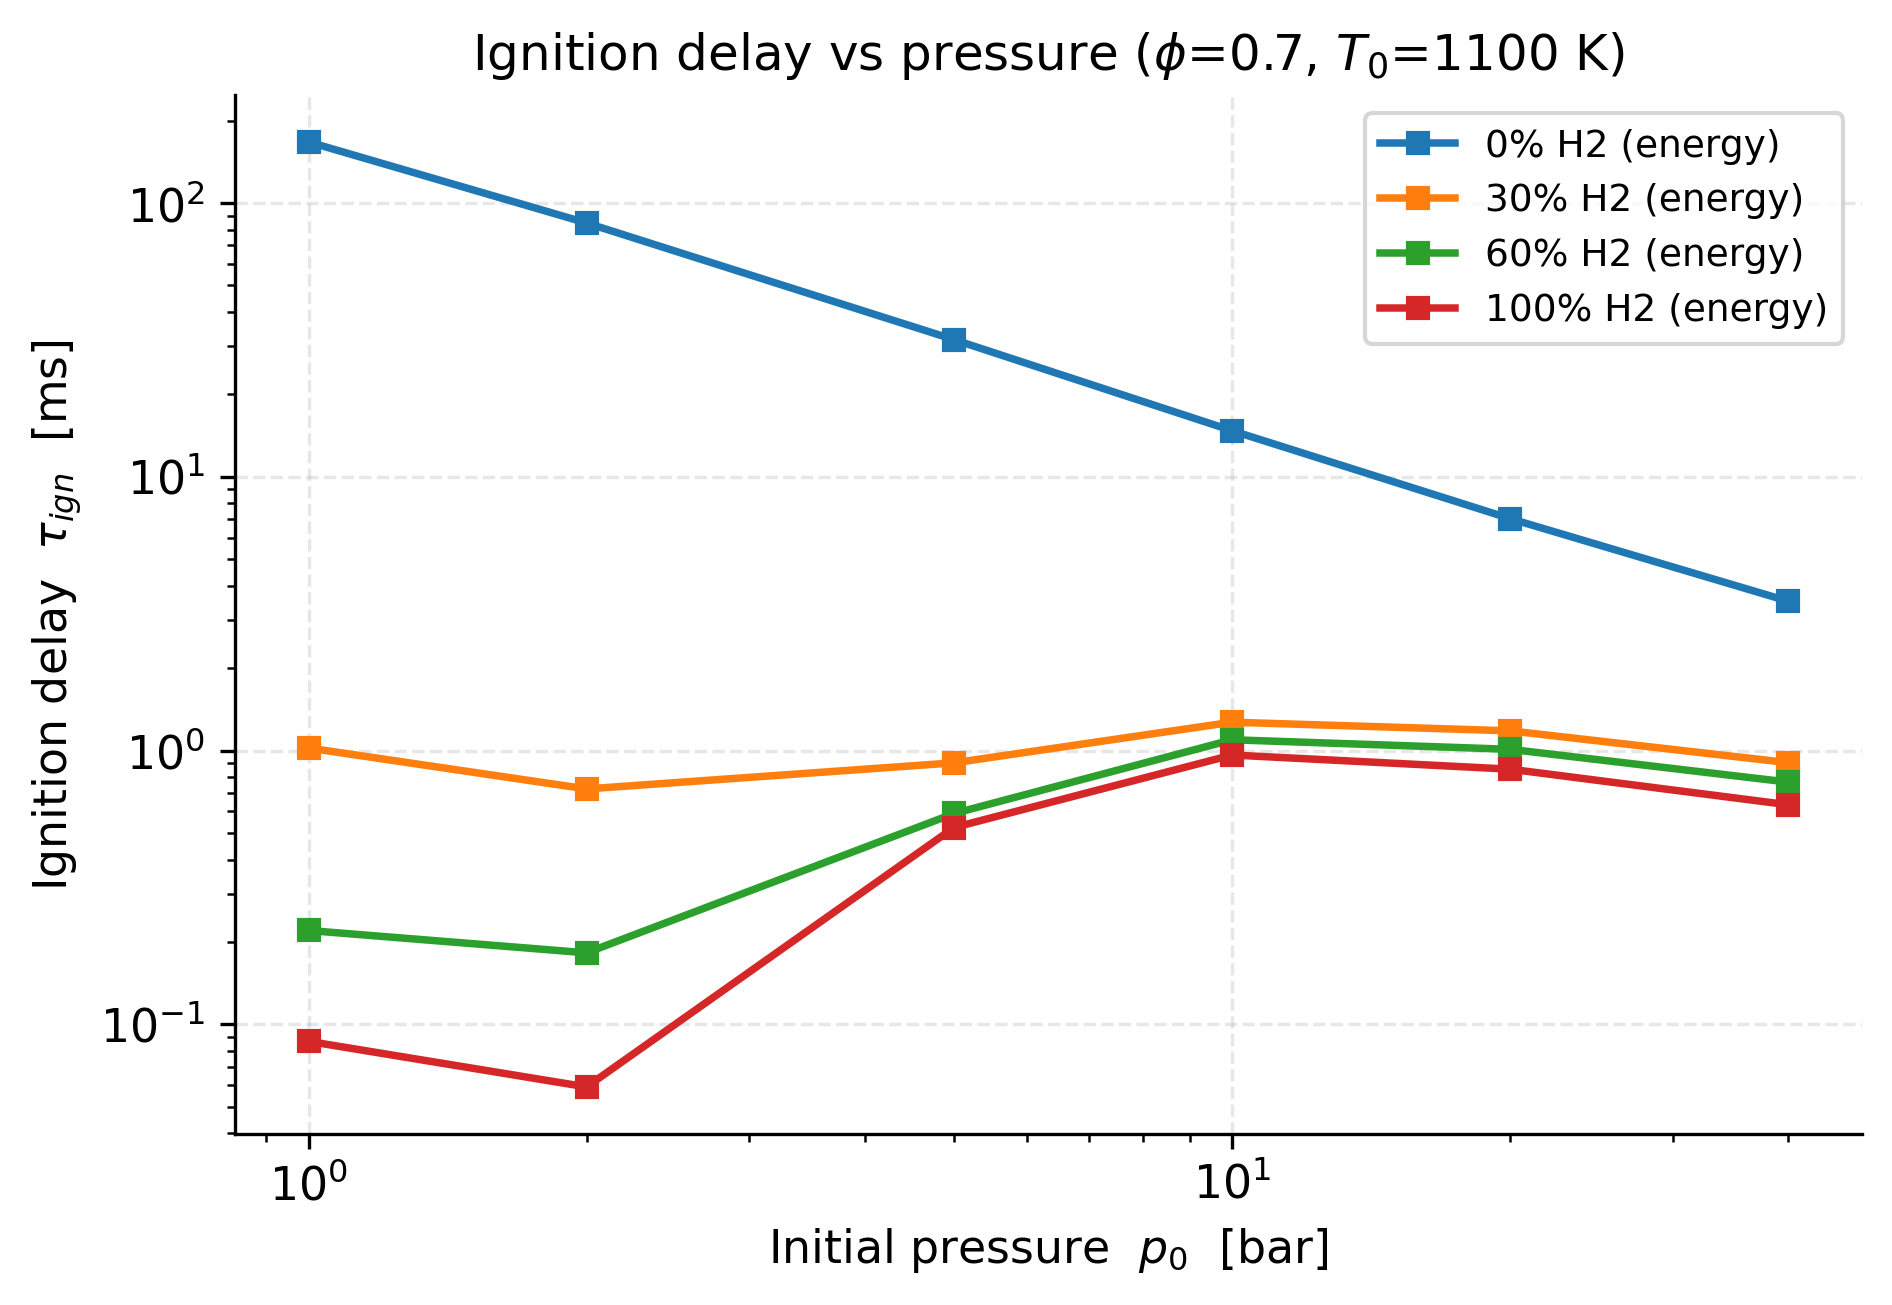
\includegraphics[width=0.78\textwidth]{figures/ignition_p_sweep.png}
\caption{Ignition delay versus initial pressure for different hydrogen energy
fractions ($\phi=0.7$, $T_0=\SI{1100}{\kelvin}$).}
\label{fig:ign-p}
\end{figure}

Figure~\ref{fig:ign-h2} isolates the effect of hydrogen at fixed temperature
and pressure. The ignition delay drops steeply with the first few per cent of
hydrogen and then more gently: at $T_0=\SI{1100}{\kelvin}$ and
$p=\SI{20}{\bar}$ it falls from \SI{7.0}{\milli\second} for pure methane to
\SI{0.86}{\milli\second} for pure hydrogen, with most of the reduction
achieved by about \SI{20}{\percent} hydrogen energy.

\begin{figure}[h]
\centering
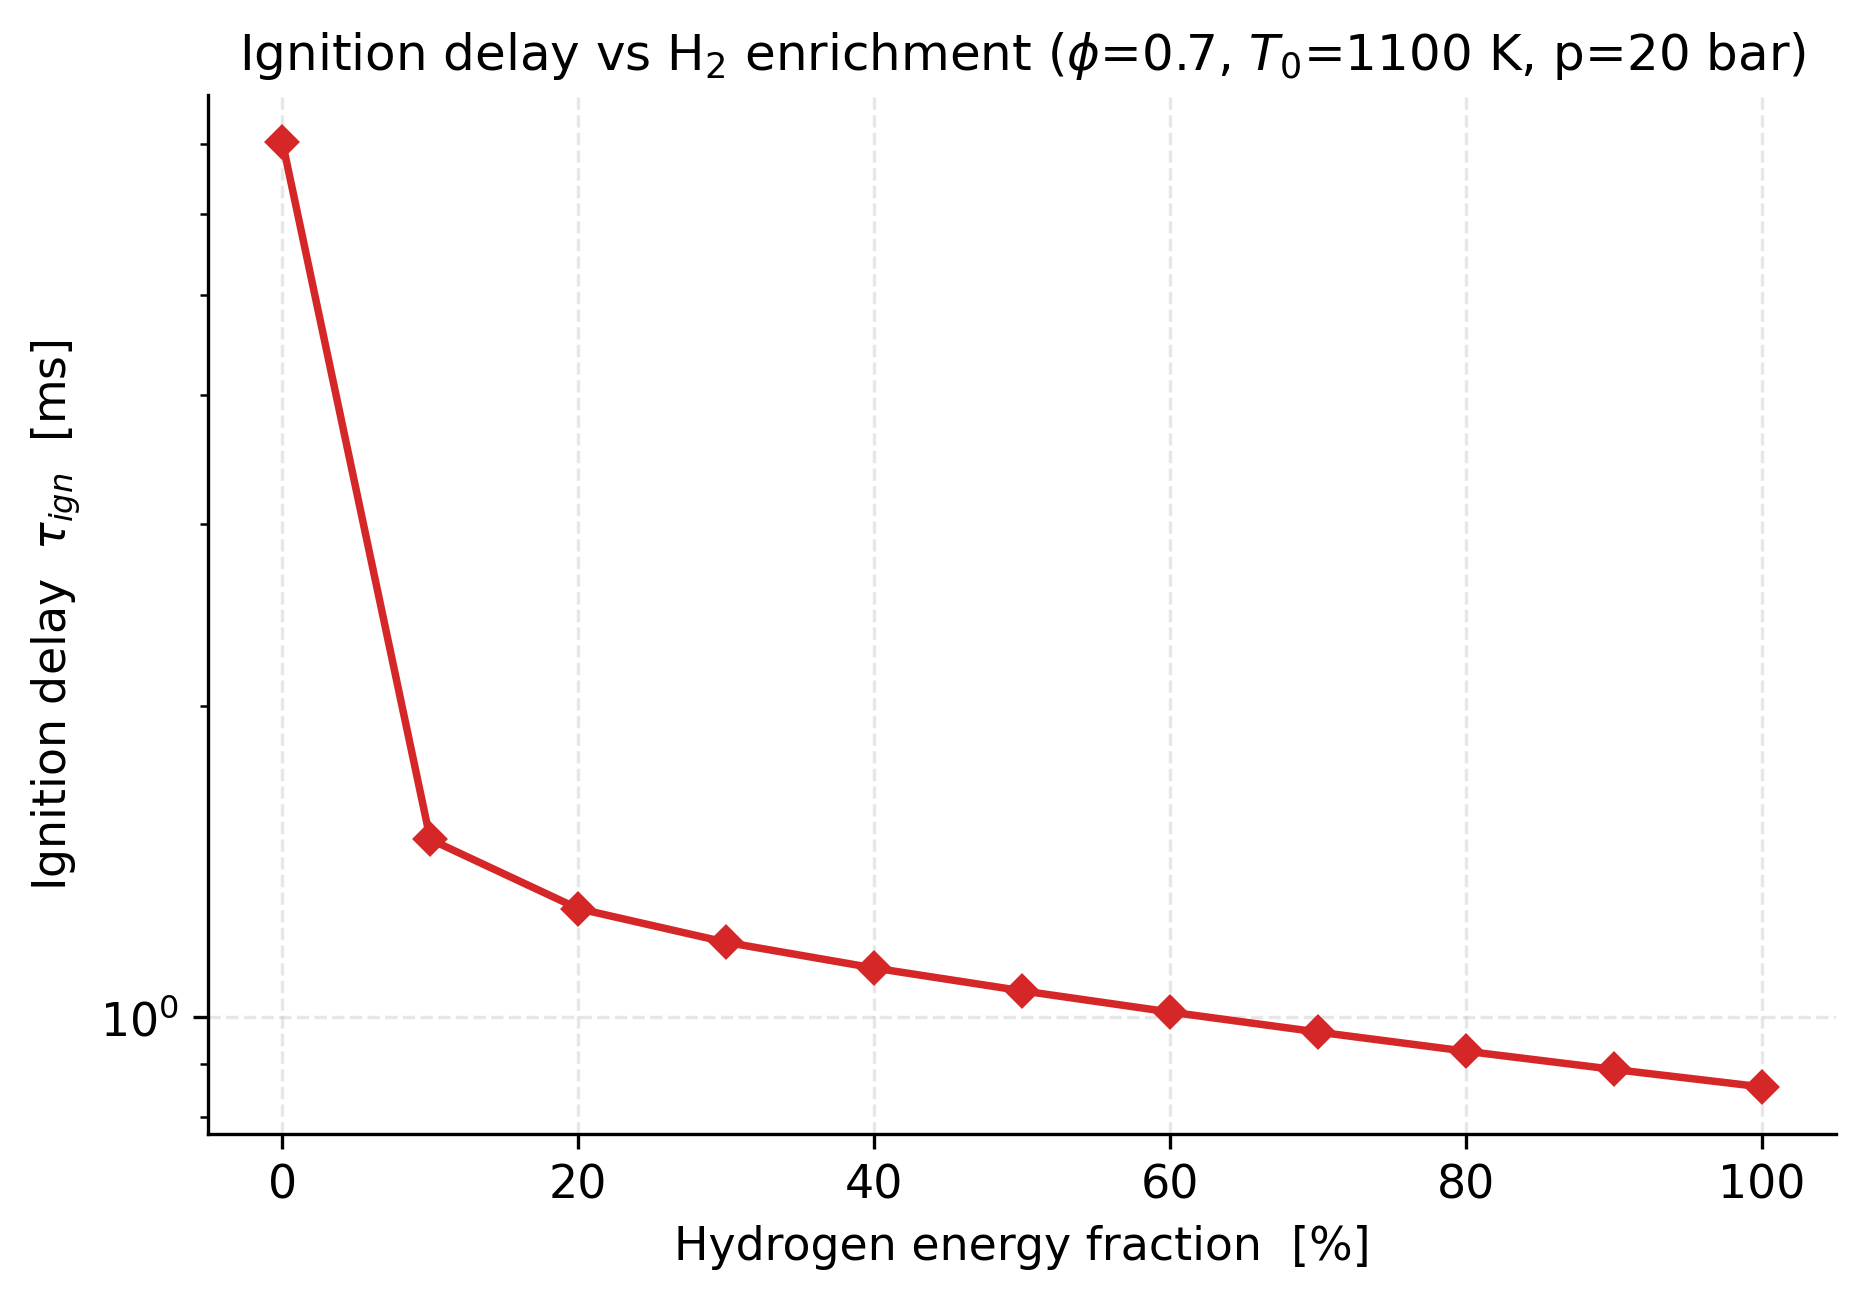
\includegraphics[width=0.78\textwidth]{figures/ignition_h2_sweep.png}
\caption{Ignition delay versus hydrogen energy fraction
($\phi=0.7$, $T_0=\SI{1100}{\kelvin}$, $p=\SI{20}{\bar}$).}
\label{fig:ign-h2}
\end{figure}

\subsection{Laminar burning velocity}

Figure~\ref{fig:flame-phi} shows the laminar burning velocity as a function of
equivalence ratio. For each blend the curve has the familiar shape with a
maximum near or slightly above stoichiometric. Hydrogen has two effects: it
raises the peak velocity dramatically and shifts the peak towards richer
mixtures. The peak burning velocity rises from about \SI{41}{\centi\meter\per
\second} for pure methane to roughly \SI{169}{\centi\meter\per\second} at
\SI{60}{\percent} hydrogen and well above \SI{500}{\centi\meter\per\second}
for pure hydrogen.

\begin{figure}[h]
\centering
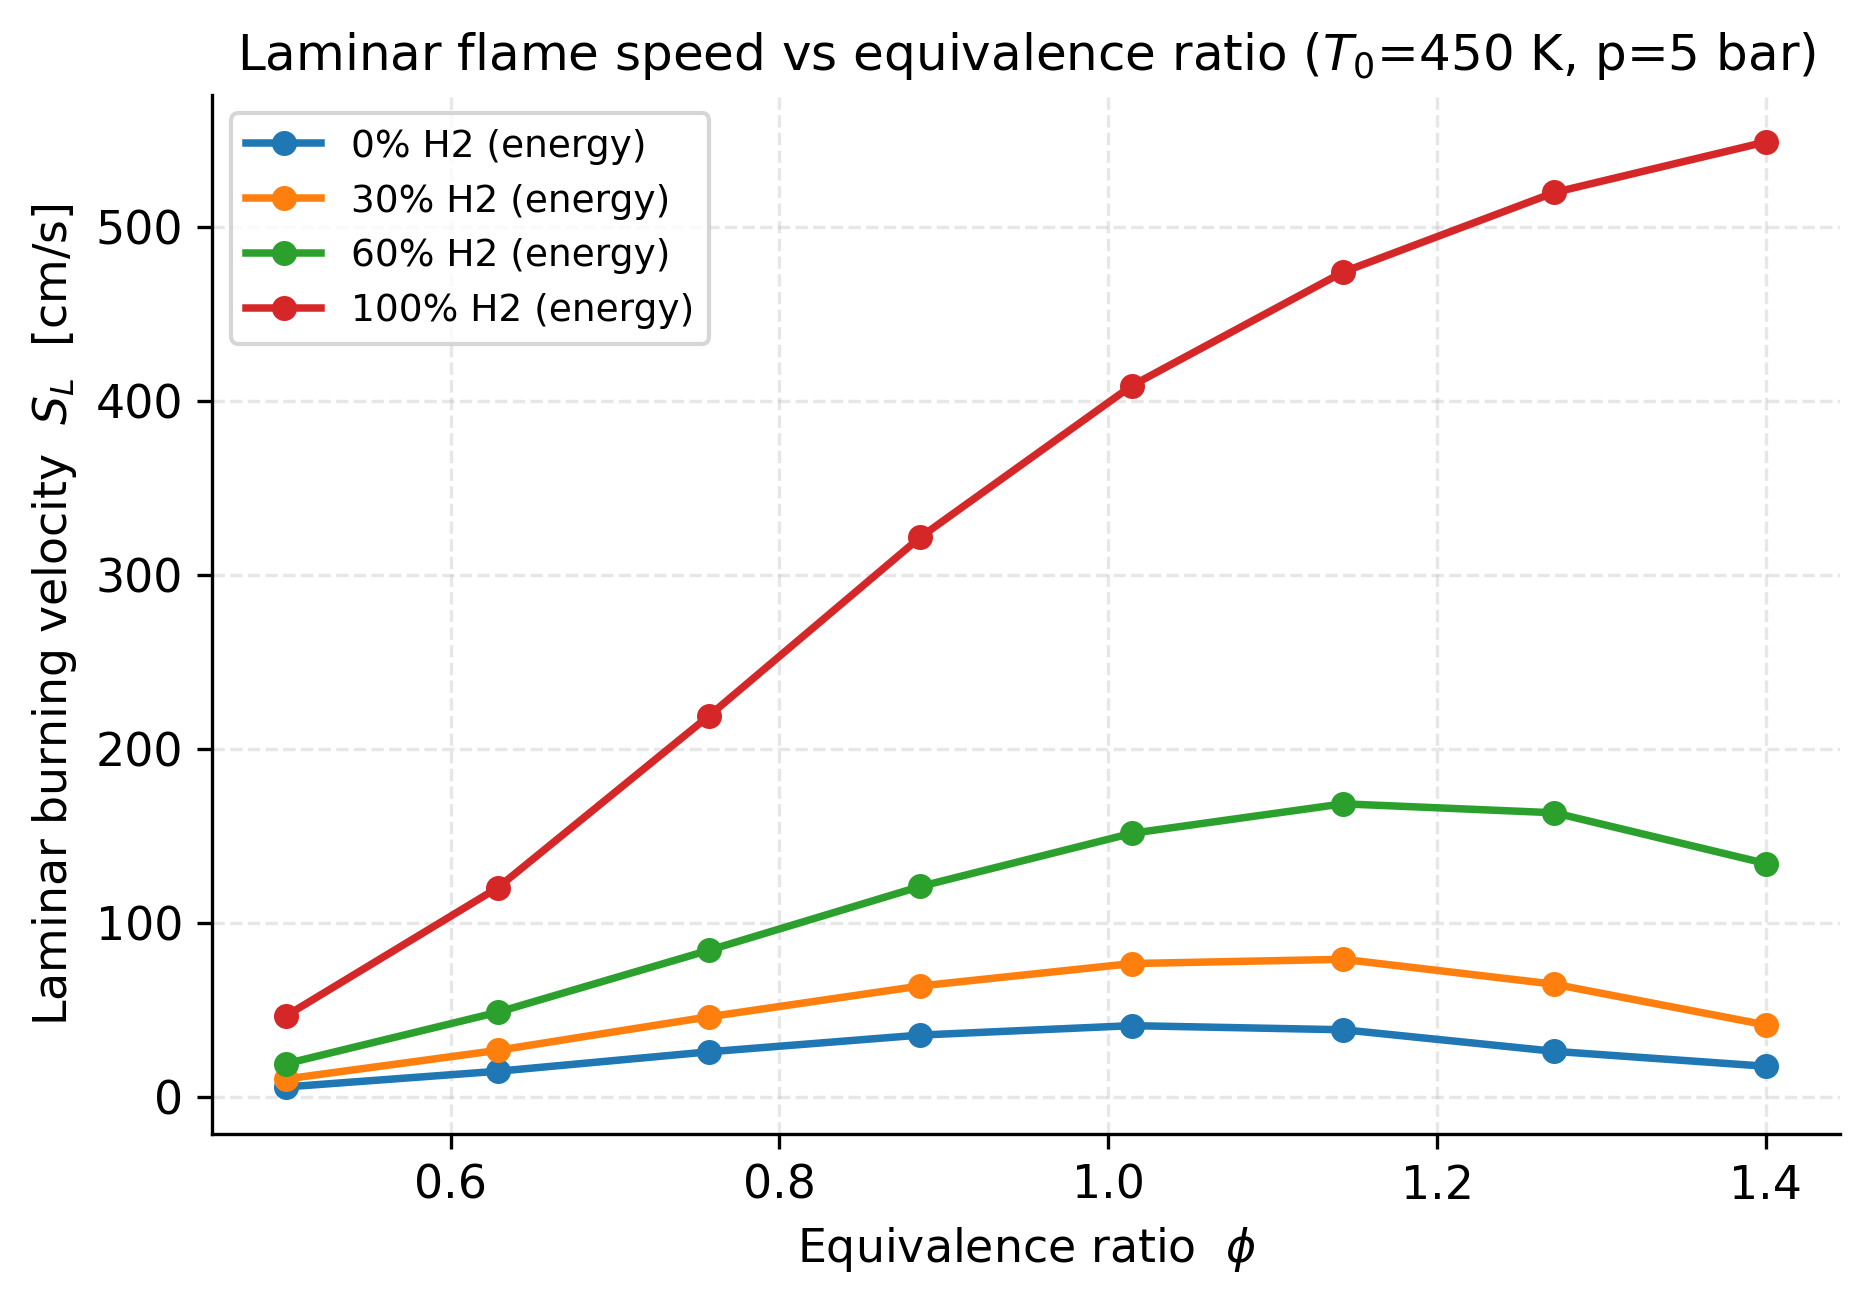
\includegraphics[width=0.78\textwidth]{figures/flame_speed_phi.png}
\caption{Laminar burning velocity versus equivalence ratio for different
hydrogen energy fractions ($T_0=\SI{450}{\kelvin}$, $p=\SI{5}{\bar}$).}
\label{fig:flame-phi}
\end{figure}

Figure~\ref{fig:flame-h2} shows the burning velocity at stoichiometric
conditions as a function of hydrogen fraction. The growth is strongly
non-linear: $S_L$ accelerates as the hydrogen content increases, reflecting
the increasing dominance of the fast hydrogen chemistry and the higher flame
temperature.

\begin{figure}[h]
\centering
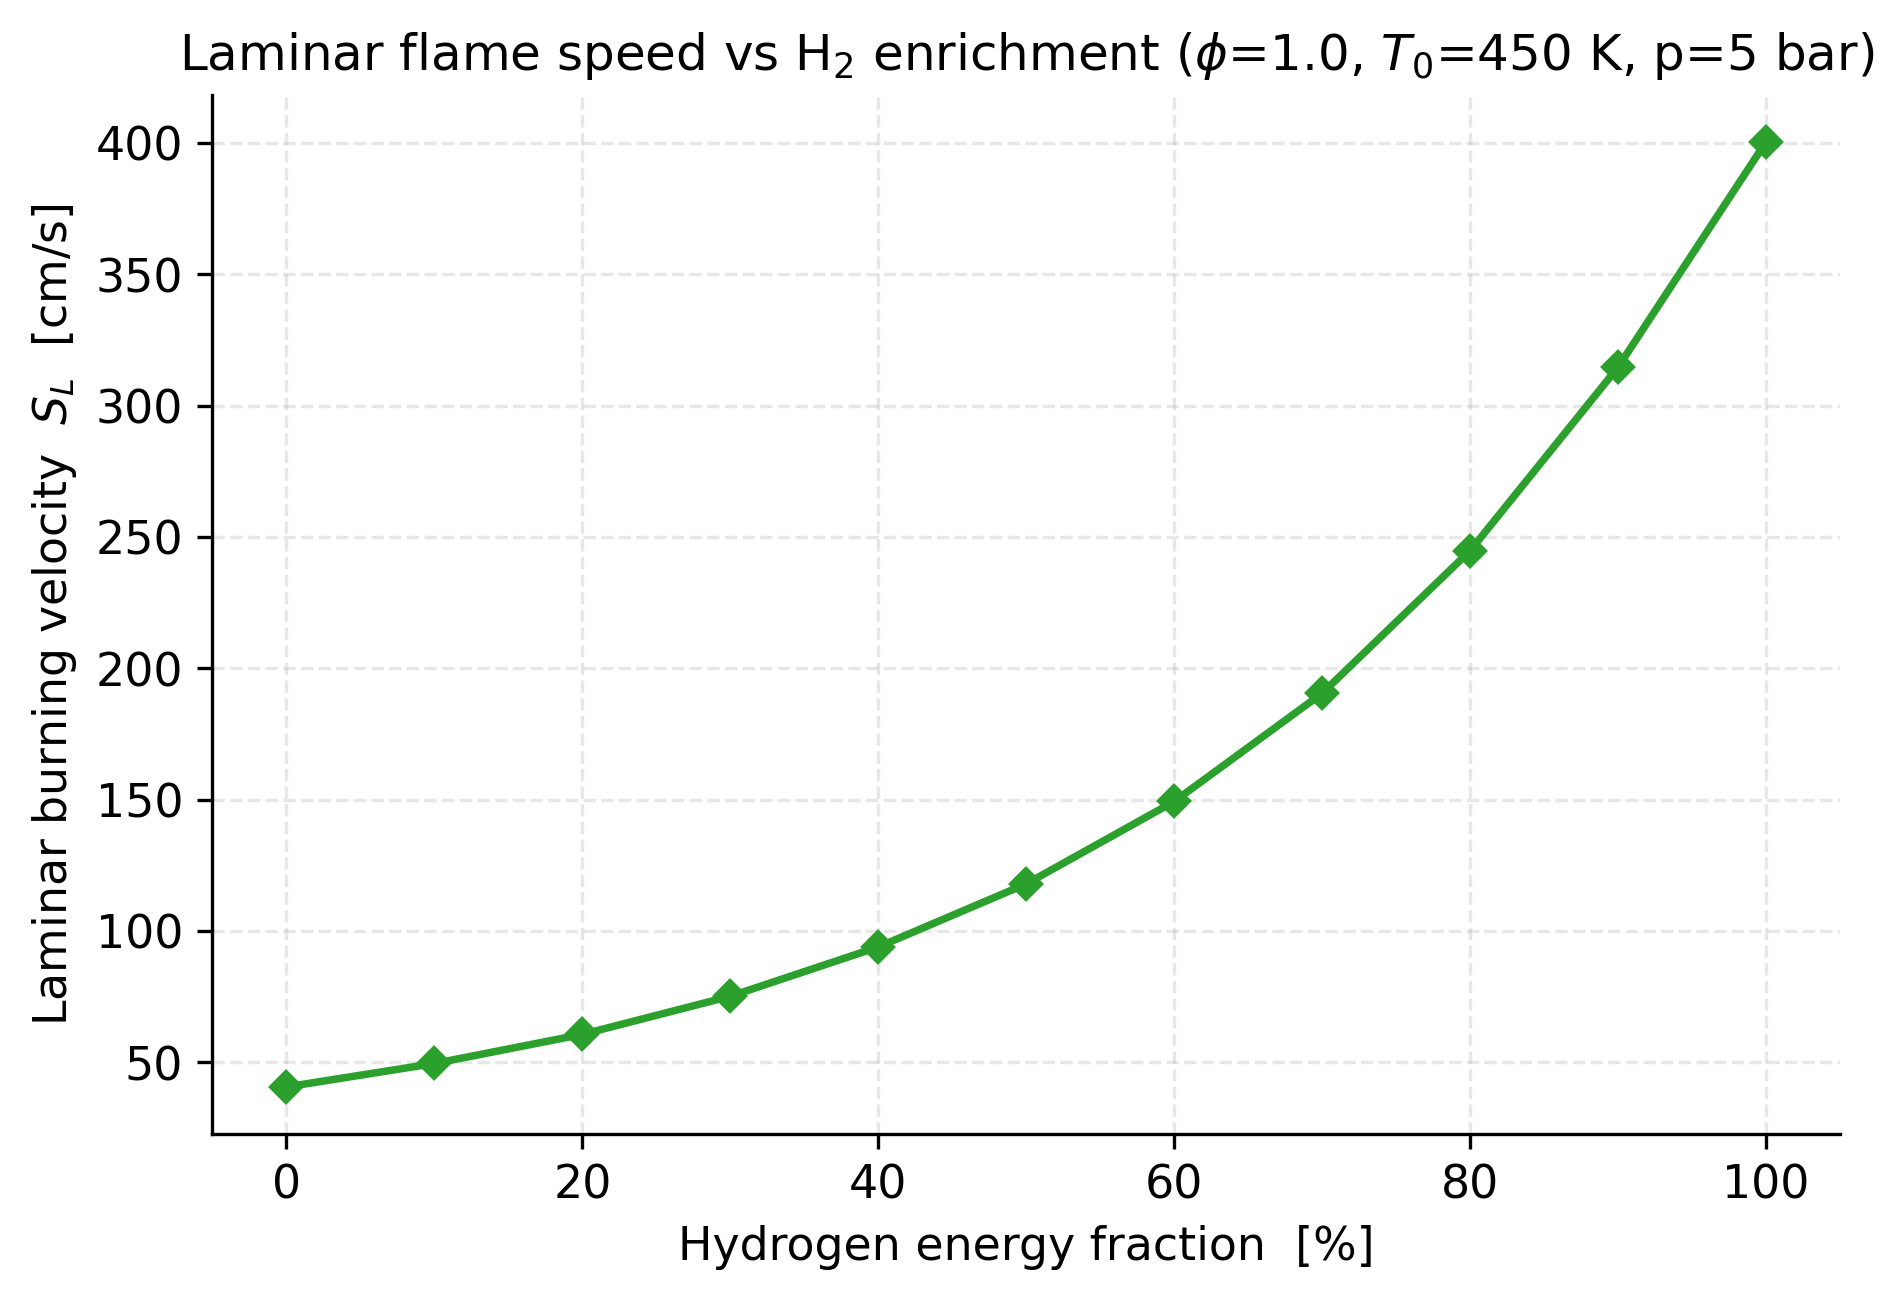
\includegraphics[width=0.78\textwidth]{figures/flame_speed_h2.png}
\caption{Laminar burning velocity versus hydrogen energy fraction at
stoichiometric conditions ($\phi=1.0$, $T_0=\SI{450}{\kelvin}$,
$p=\SI{5}{\bar}$).}
\label{fig:flame-h2}
\end{figure}

\subsection{NO\textsubscript{x} emissions}

Figure~\ref{fig:nox-phi} shows the NO\textsubscript{x} emission index as a
function of equivalence ratio. Each curve has a pronounced maximum at a
slightly lean to near-stoichiometric mixture and falls off steeply on either
side, the classical thermal-NO\textsubscript{x} bell shape driven by the
exponential temperature dependence of the Zeldovich route. Hydrogen shifts the
whole family of curves upward: the peak emission index grows from about
\SI{101}{\gram\per\kilogram} for pure methane to over
\SI{460}{\gram\per\kilogram} for pure hydrogen.

\begin{figure}[h]
\centering
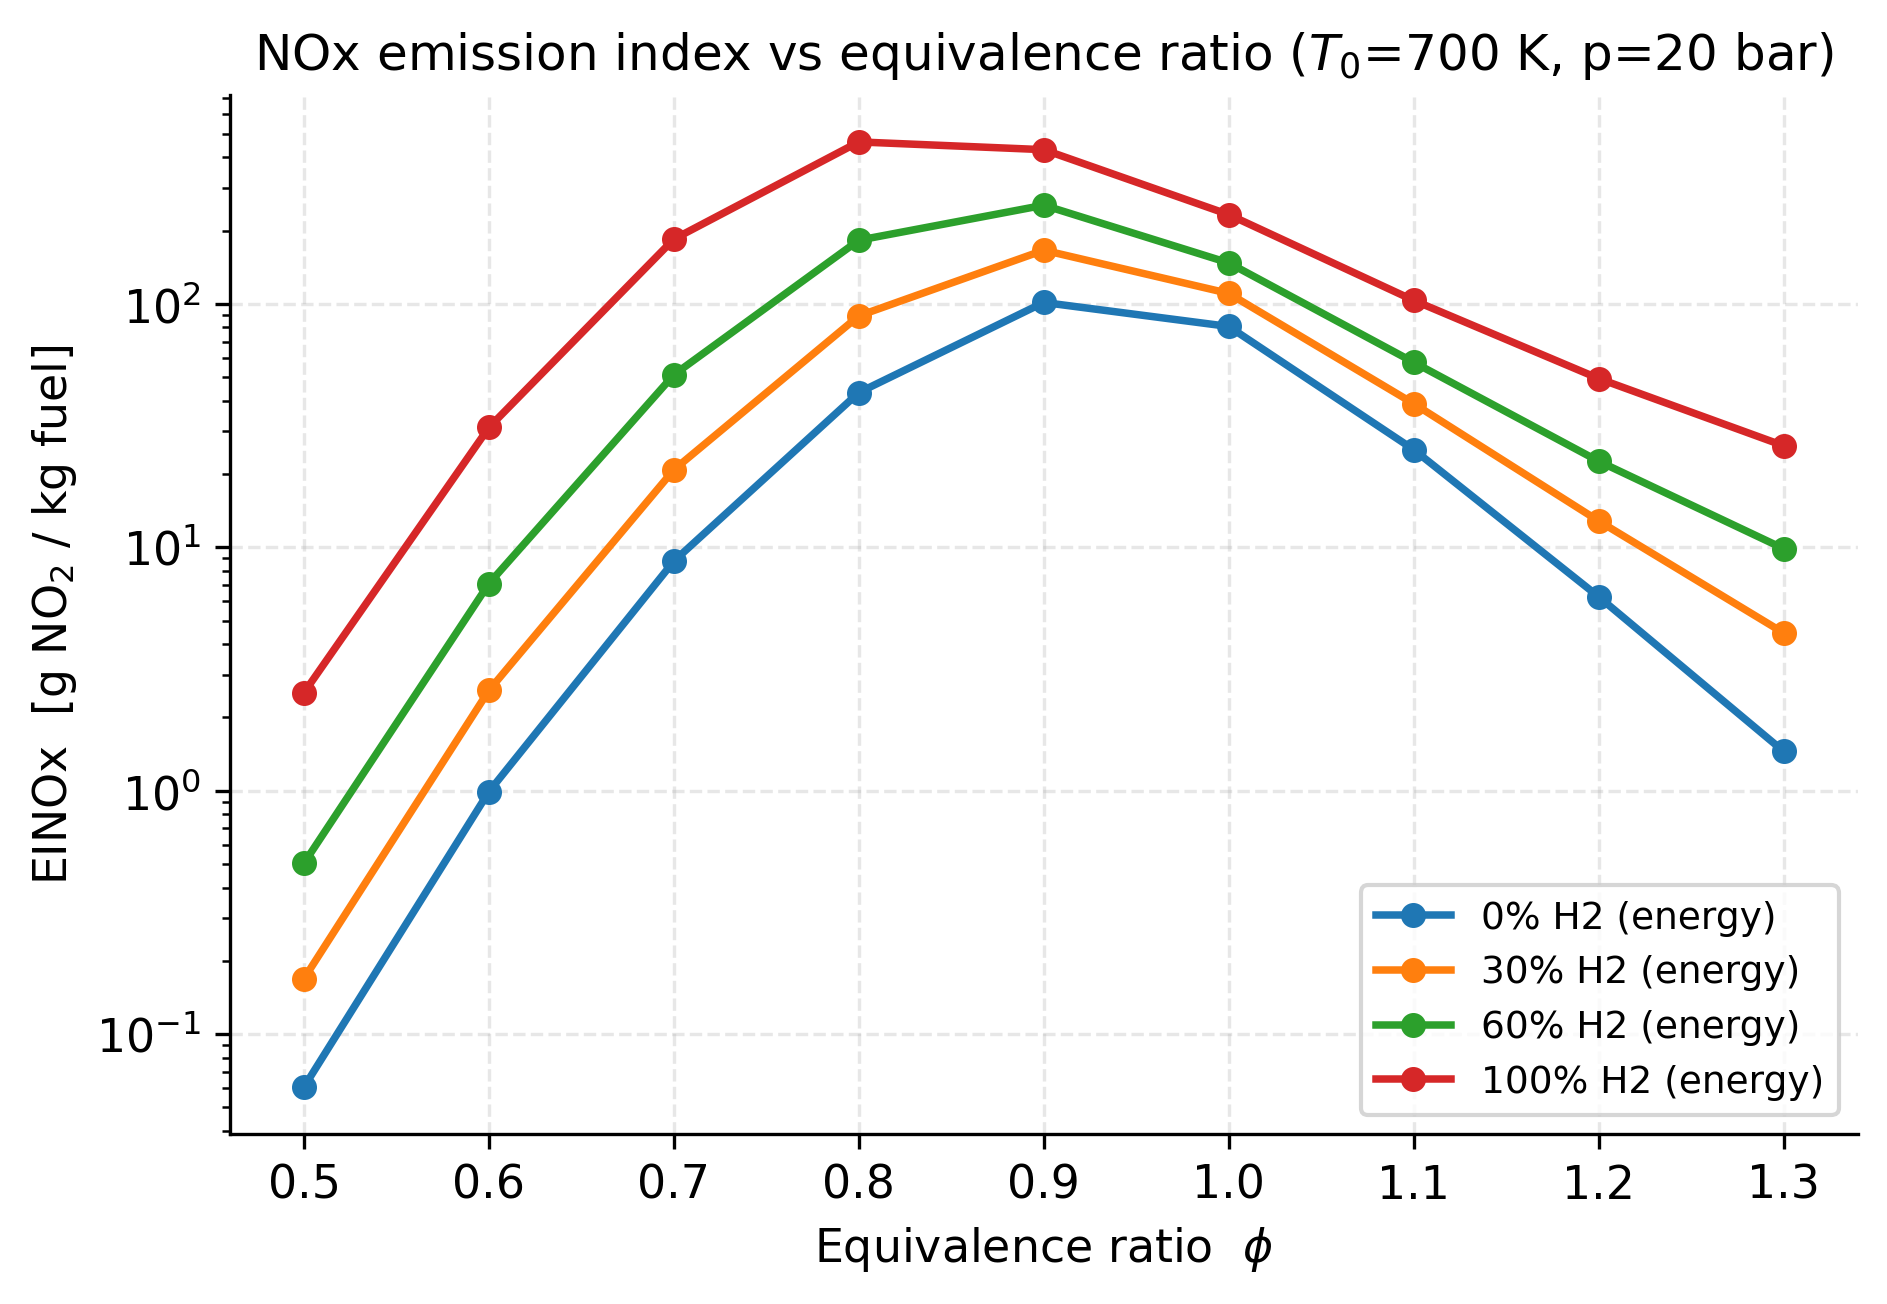
\includegraphics[width=0.78\textwidth]{figures/nox_phi.png}
\caption{NO\textsubscript{x} emission index versus equivalence ratio for
different hydrogen energy fractions ($T_0=\SI{700}{\kelvin}$,
$p=\SI{20}{\bar}$).}
\label{fig:nox-phi}
\end{figure}

The adiabatic flame temperature behind these emissions is shown in
Figure~\ref{fig:tad-phi}. It rises with hydrogen content at every equivalence
ratio, which is the proximate cause of the higher NO\textsubscript{x}.

\begin{figure}[h]
\centering
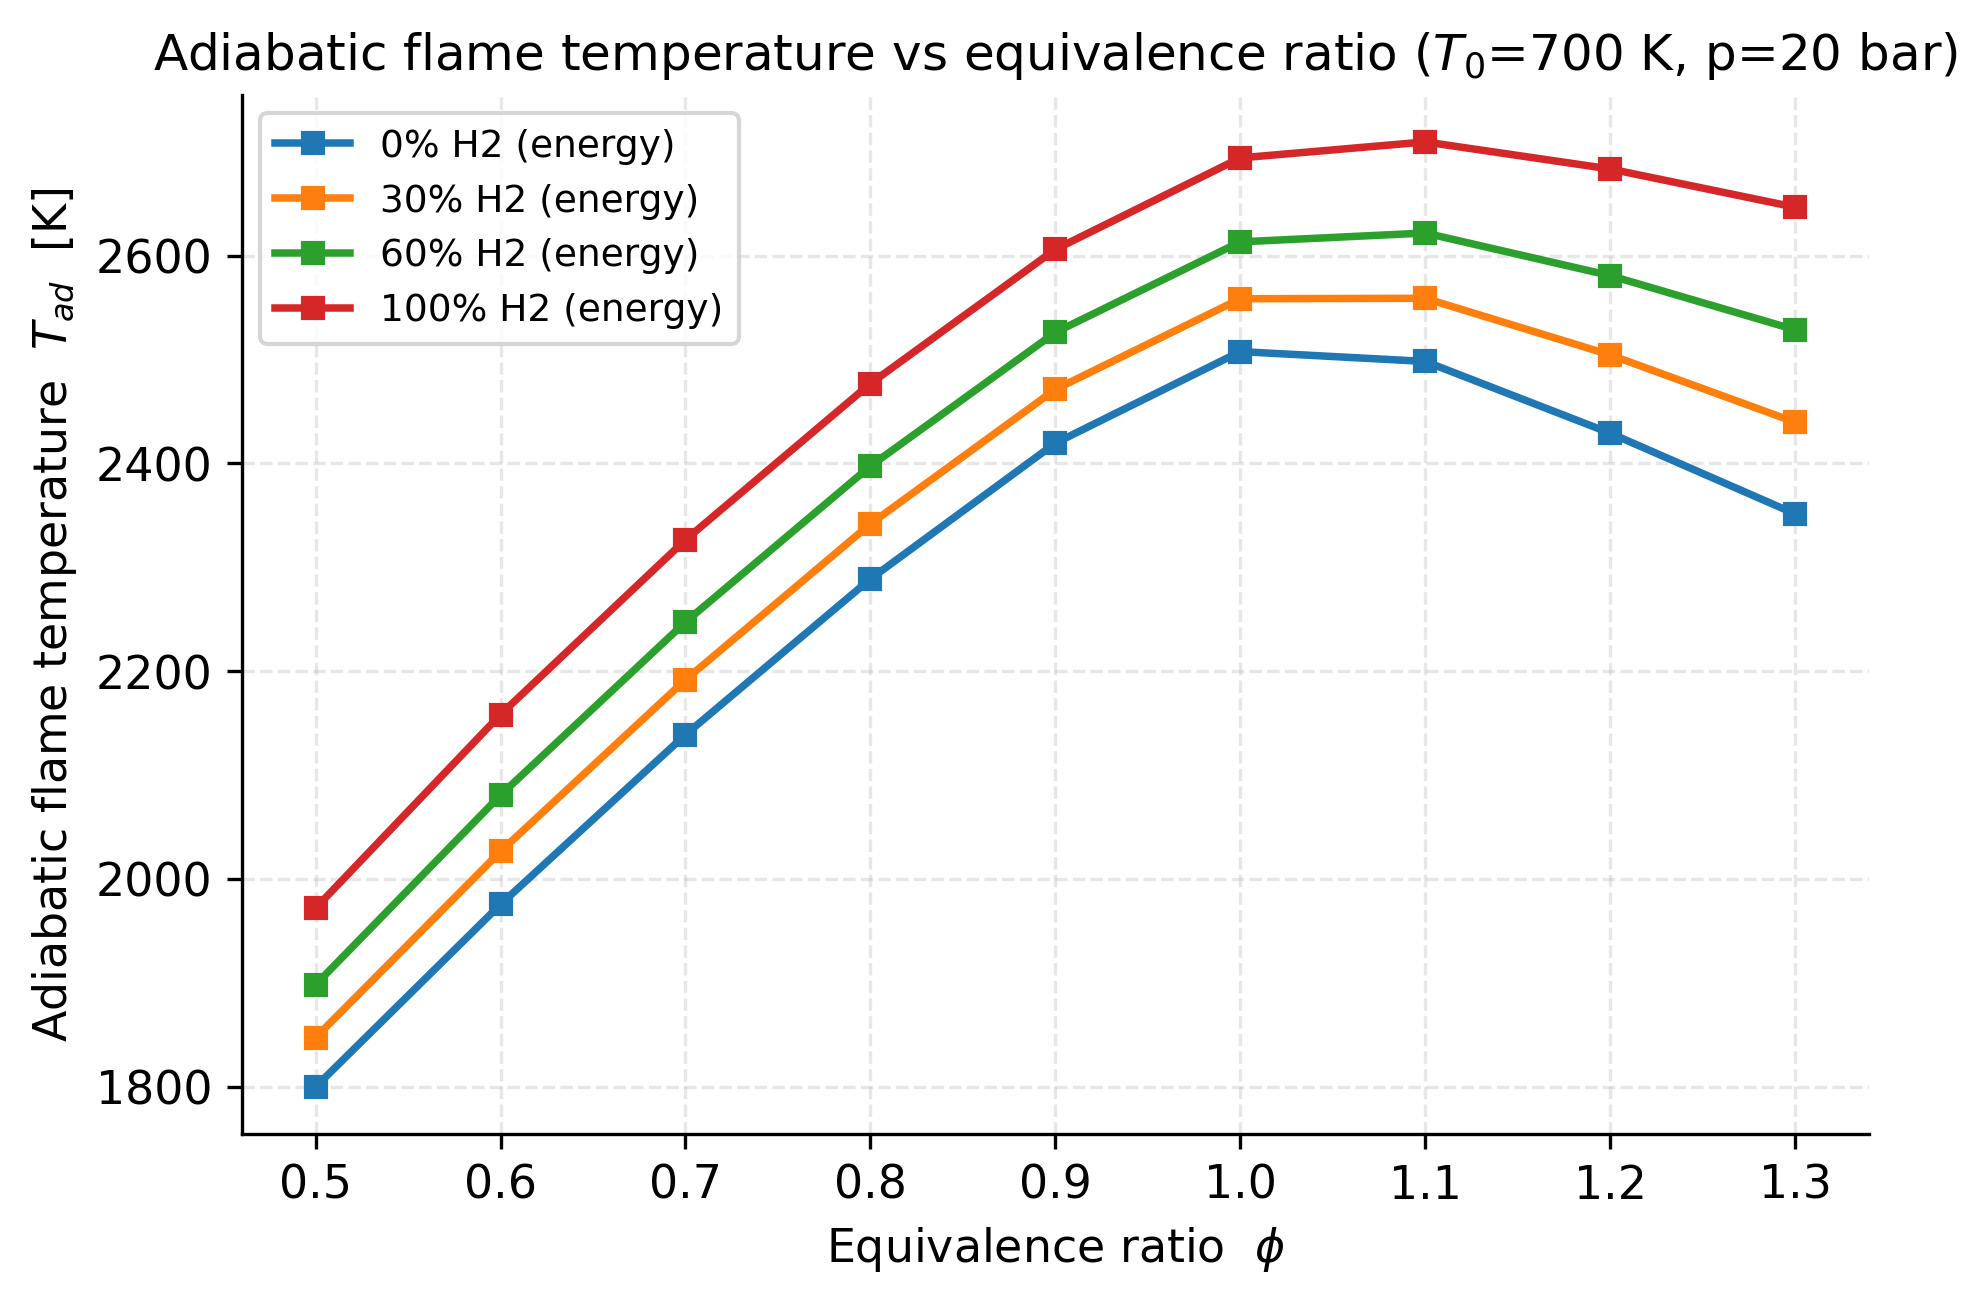
\includegraphics[width=0.78\textwidth]{figures/tad_phi.png}
\caption{Adiabatic flame temperature versus equivalence ratio for different
hydrogen energy fractions ($T_0=\SI{700}{\kelvin}$, $p=\SI{20}{\bar}$).}
\label{fig:tad-phi}
\end{figure}

The central trade-off of hydrogen enrichment is made explicit in
Figure~\ref{fig:nox-h2}, which plots the emission index and the flame
temperature together against the hydrogen fraction at a fixed lean condition
($\phi=0.7$). As the hydrogen energy fraction goes from \SI{0}{} to
\SI{100}{\percent} the flame temperature rises by only about
\SI{190}{\kelvin}, from \SI{2139}{\kelvin} to \SI{2327}{\kelvin}, while the
emission index increases by more than a factor of twenty, from
\SI{8.8}{\gram\per\kilogram} to \SI{185}{\gram\per\kilogram}. The flame
temperature rises almost linearly, but the NO\textsubscript{x} responds
exponentially, which is exactly the expected signature of thermal
NO\textsubscript{x}.

\begin{figure}[h]
\centering
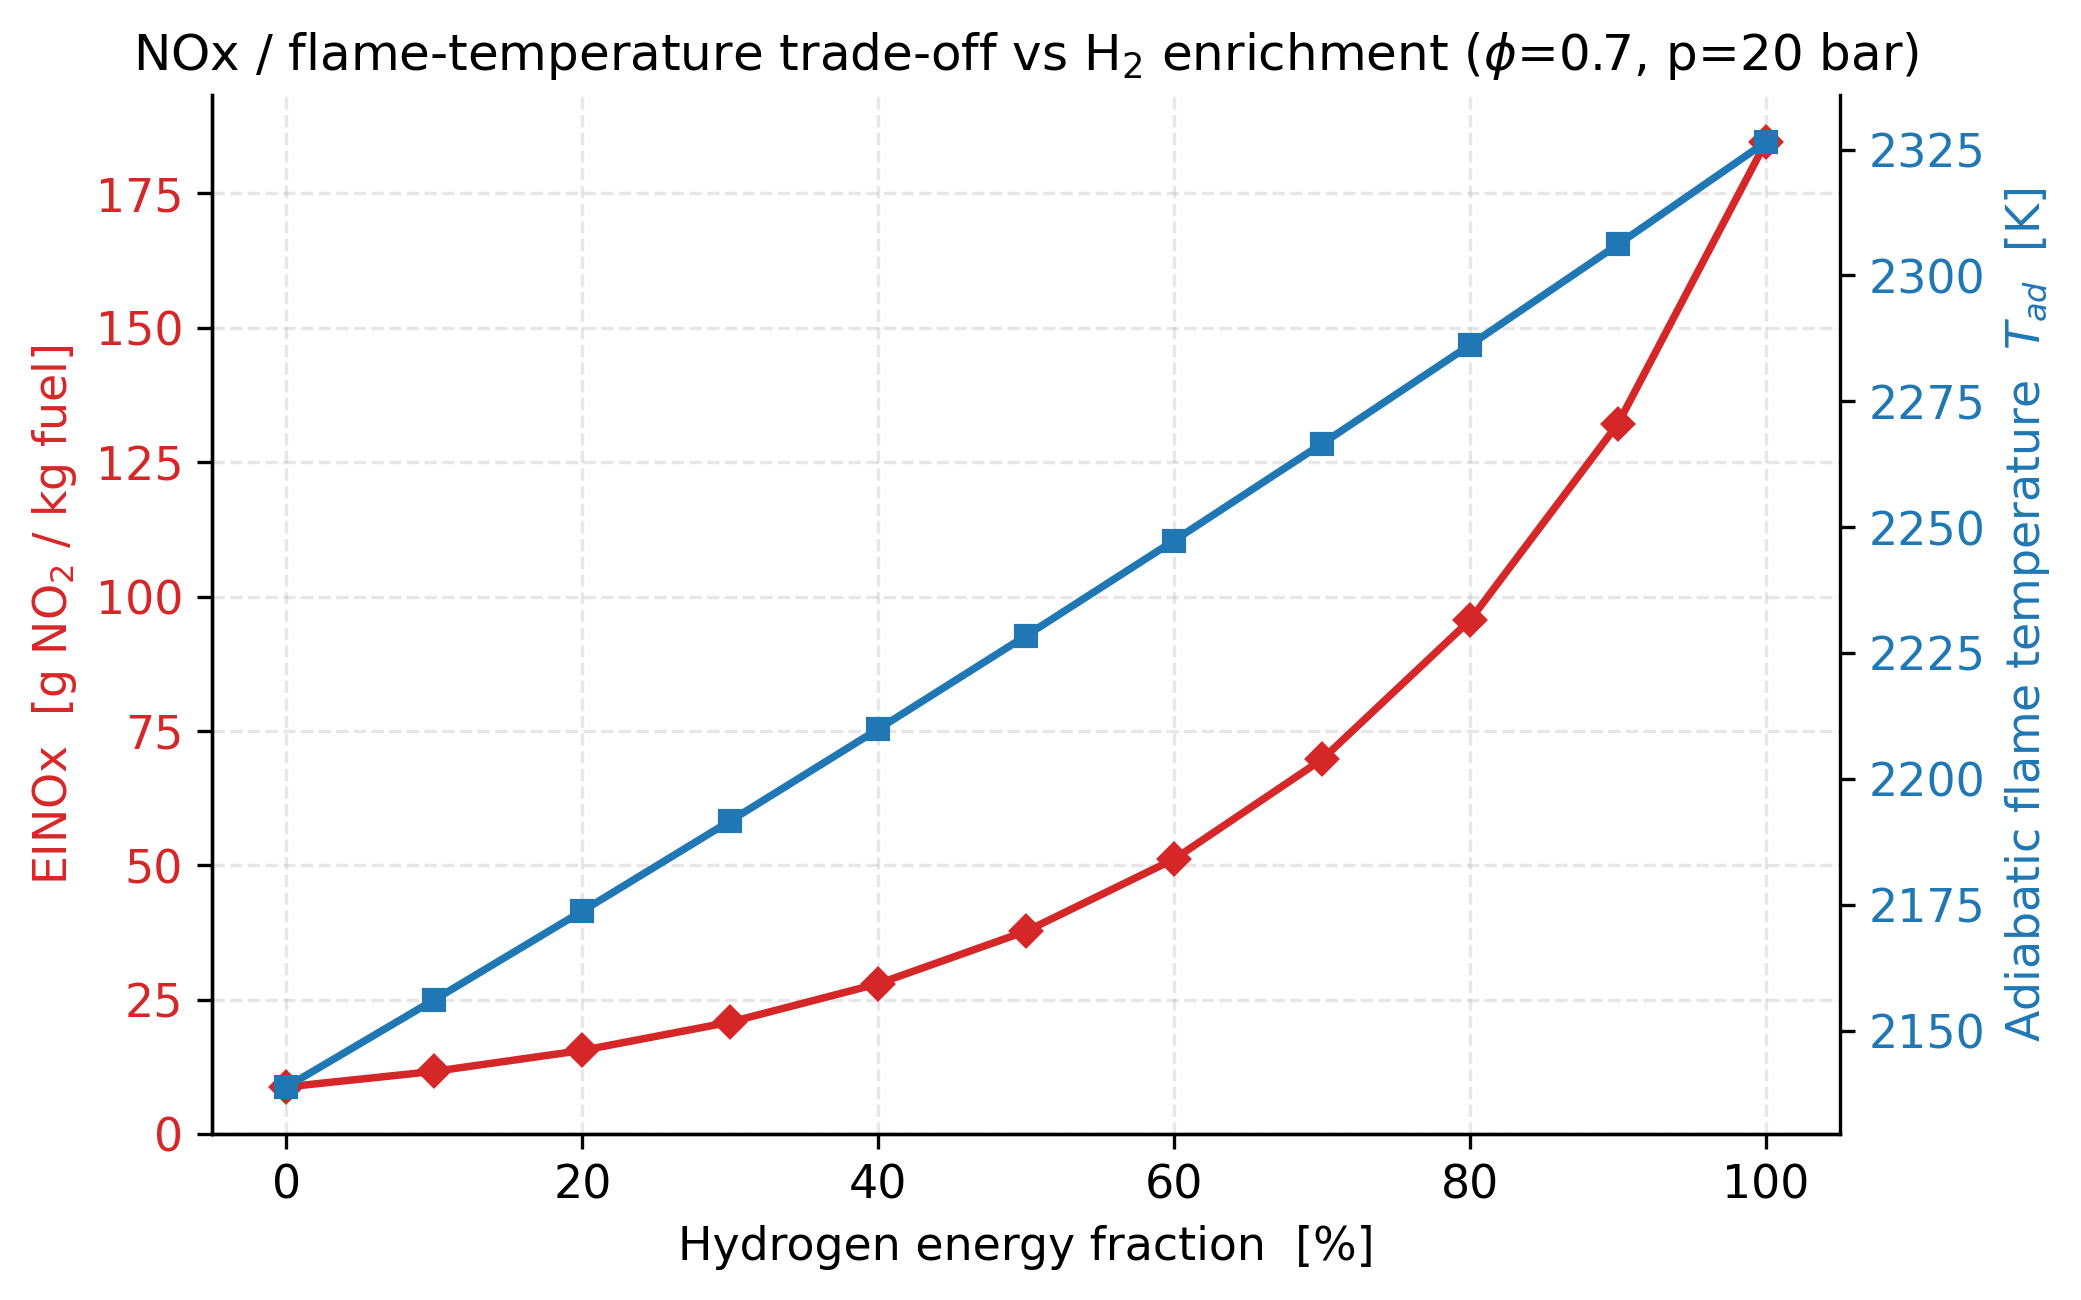
\includegraphics[width=0.80\textwidth]{figures/nox_h2.png}
\caption{NO\textsubscript{x} emission index and adiabatic flame temperature
versus hydrogen energy fraction at a lean condition
($\phi=0.7$, $p=\SI{20}{\bar}$).}
\label{fig:nox-h2}
\end{figure}

\subsection{Mechanism validation}
\label{sec:validation}

Because GRI-Mech~3.0 is optimised mainly for natural gas, its reliability at
the pure-hydrogen end of the blend range must be checked. The ignition delay
and the laminar burning velocity of \SI{100}{\percent} hydrogen were therefore
recomputed with a dedicated detailed \ce{H2}/\ce{O2} mechanism (10 species, 29
reactions) and overlaid on the GRI-Mech results in Figure~\ref{fig:mech}. The
agreement is excellent: the ignition delay differs by less than
\SI{0.1}{\percent} across the temperature range, and the laminar burning
velocity by at most \SI{3.2}{\percent}, with the largest deviation at the lean
limit where the hydrogen chemistry is most sensitive. This confirms that
GRI-Mech~3.0 is an appropriate single mechanism for the whole blend range.

\begin{figure}[h]
\centering
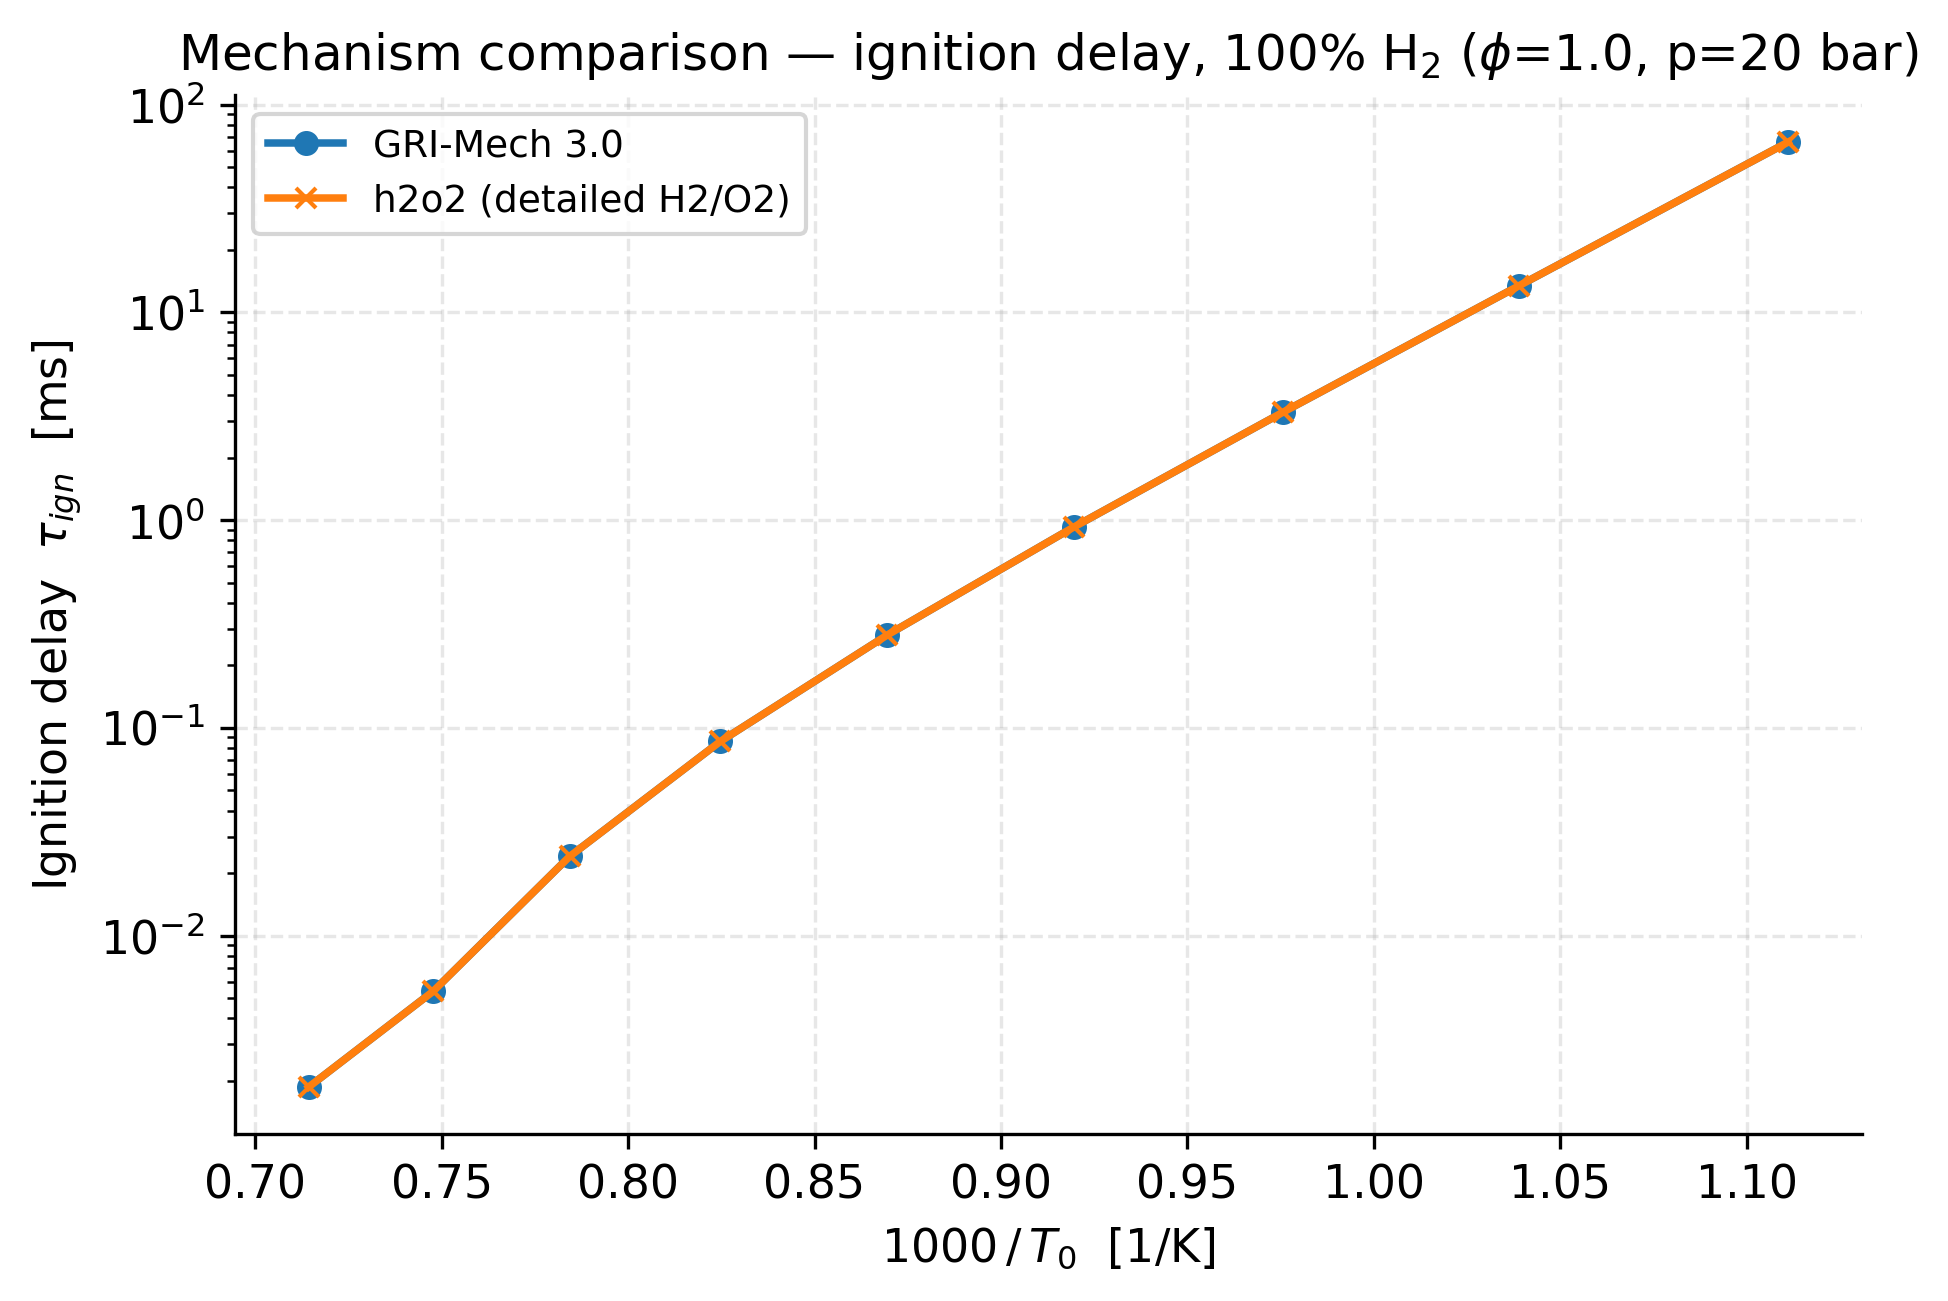
\includegraphics[width=0.49\textwidth]{figures/mech_comparison_ignition.png}
\hfill
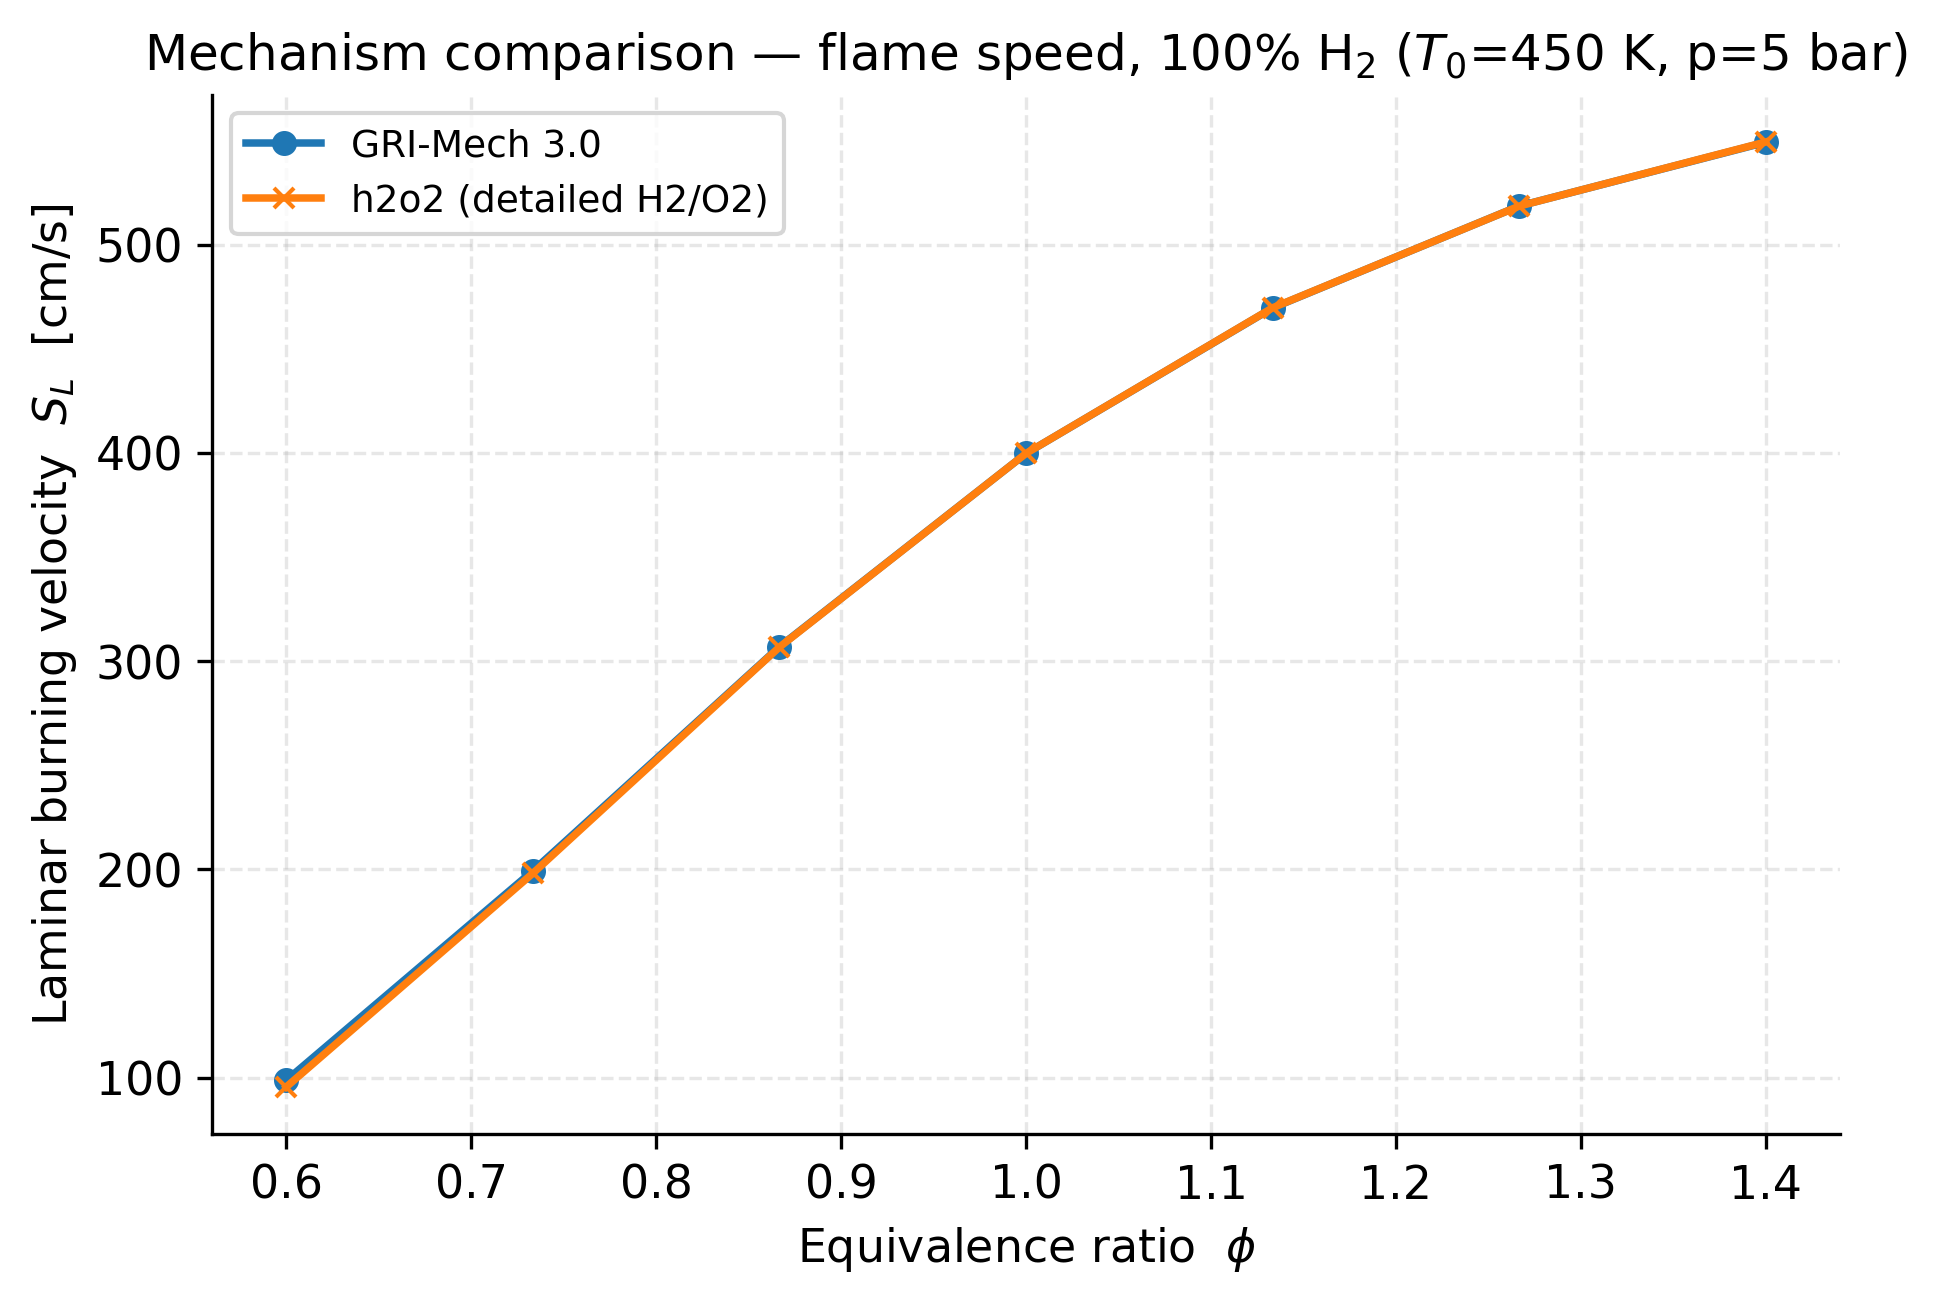
\includegraphics[width=0.49\textwidth]{figures/mech_comparison_flame.png}
\caption{Mechanism validation for \SI{100}{\percent} hydrogen: ignition delay
(left) and laminar burning velocity (right), GRI-Mech~3.0 versus a detailed
\ce{H2}/\ce{O2} mechanism.}
\label{fig:mech}
\end{figure}

% ===========================================================================
% 5. Conclusions
% ===========================================================================
\section{Conclusions}

The effect of hydrogen enrichment on methane--air combustion was computed with
Cantera and GRI-Mech~3.0 over the full blend range, under conditions
representative of an aero gas turbine combustor. The main findings are as
follows.

Hydrogen substantially improves the ignition and burning characteristics. The
ignition delay falls by almost an order of magnitude from pure methane to pure
hydrogen, with most of the benefit obtained at modest hydrogen fractions, and
the laminar burning velocity increases strongly and non-linearly, by roughly an
order of magnitude at stoichiometric conditions. Both effects are favourable
for relight, flame stabilisation and a compact reaction zone.

These benefits come at the cost of NO\textsubscript{x}. Because hydrogen raises
the adiabatic flame temperature and thermal NO\textsubscript{x} depends
exponentially on temperature, a modest temperature rise produces a large
emission penalty: at a lean condition the emission index increased more than
twentyfold across the blend range for only a \SI{190}{\kelvin} rise in flame
temperature. Lean operation remains the principal means of keeping
NO\textsubscript{x} acceptable, and it becomes more important, not less, as the
hydrogen fraction increases.

Finally, the use of a single mechanism across the whole blend range was
justified: GRI-Mech~3.0 reproduces the predictions of a dedicated detailed
hydrogen mechanism for both ignition delay and flame speed of pure hydrogen to
within a few per cent. Overall, hydrogen enrichment is an effective route to
decarbonising gas turbine combustion, but it shifts the design point firmly
towards lean, carefully temperature-controlled operation in order to manage the
NO\textsubscript{x} trade-off.

\end{document}
